\section{Non-Tabular Model-Free RL}

\begin{definition}[Idea]
    Approx \(V, Q\) without \(\OB(n), \OB(nm)\) space.
\end{definition}

% stochastic gradient descent with a bootstrapping estimate is also called stochastic-semi-gradient descent.
\begin{definition}[TD as SGD]
    \resizebox{0.72\linewidth}{!}{
    \(l_2(\TH; x, r, x') = \frac{1}{2} (r + \gamma \TH^{\text{old}}(x') - \TH(x))^2\)
    }
\end{definition}

% \begin{itemize}[leftmargin=*]
%     \item \(\delta_{\text{TD}} = r + \gamma \TH^{\text{old}}(x') - \TH(x)\)

% \end{itemize}


\begin{definition}[Q-Learn. w/ F.A.]
    \(\TH \leftarrow \TH - \alpha_t \delta_* \nabla_{\TH} Q^\star(x, a;\TH)\)
    Upd. \(\TH^{\text{old}}\) aft. \(|\D|\) stp. \(l_2(\TH) = \frac{1}{2}\sum_{d \in \D}(\delta_*(d))^2\)
    \begin{itemize}[leftmargin=*]
        \item \hspace{-2pt}\resizebox{1.01\linewidth}{!}{
        \(\delta_{\text{DQN}} = { r + \gamma \max_{a'} Q^\star(x', a'; \TH^{\text{old}}) - Q^\star(x, a; \TH)}\)
        } \\ % note that the update of the online-network still happens with a random sample of the replay buffer. the summation is implicit.
        Use replay buf. for training. Maintain data of transitions. Clone/fix network accross epis.
        \item \hspace{-2pt}\resizebox{1.01\linewidth}{!}{
        \(\delta_{\text{DDQN}} = { r + \gamma Q^\star(x', a^\star(x';\TH); \TH^{\text{old}}) - Q^\star(x, a; \TH)}\)
        } \\
        where \(a^\star(x'; \TH) = \argmax{a'}Q^\star(x', a';\TH)\)
    \end{itemize}
\end{definition}

\subsection{Policy Gradient Methods \(\pi^\star(x) \approx \pi_\varphi(x)\)}
\begin{center}
    \(j(\pi) = \E_\pi[G_0], \quad \nabla_\varphi j(\varphi) \approx {\color{H2}\nabla_\varphi \E_{\tau \sim \Pi_\varphi}[G_0]}\) \\
    \(\Pi_\varphi(\tau) = p(x_0) \Pi_{t=0}^{T-1} \pi_\varphi(a_t \mid x_t) p(x_{t+1} \mid x_t, a_t)\)
\end{center}

\begin{definition}[Score-Gr-Est]
    \({\color{H2} \E_{\tau \sim \Pi_\varphi}[(G_0{\color{gray}- b})\nabla_\varphi \log \Pi_\varphi(\tau)]}\)
\end{definition}

\begin{definition}[REINFORCE]
    SGE with downstream return:
    \(\varphi \leftarrow \varphi + \eta {\color{H2}\gamma^t g_{t:T} \nabla_\varphi \log \pi_\varphi(a_t \mid x_t)}\) using MC.
\end{definition}

\begin{definition}[Adv. F.]
    \(a^\pi(x, a) = q^\pi(x, a) - v^\pi(x)\)
\end{definition}

\begin{definition}[PG-Thm]
    Use VF-est. with PGM (online)

    % \resizebox{\linewidth}{!}{
    %     \(\nabla_\varphi j(\varphi) = \sum_{0}^\infty \E_{x_t, a_t}[\gamma^t q^{\pi_\varphi}(x_t, a_t) \nabla_\varphi \log \pi_\varphi(a_t \mid x_t)]\)
    % }
    \begin{center}
    \(\nabla_\varphi j(\varphi) = \E_{(x, a) \sim \pi_\varphi}[q^\pi_\varphi(x, a) \nabla \log \pi_\varphi(a \mid x)]\)
    \end{center}
\end{definition}

\subsection{Actor-Critic}
\begin{center}
    \textit{Actor} (\(\pi\)-app. [PG-T]), \textit{Critic} (\(Q\)-app. [TD])
\end{center}

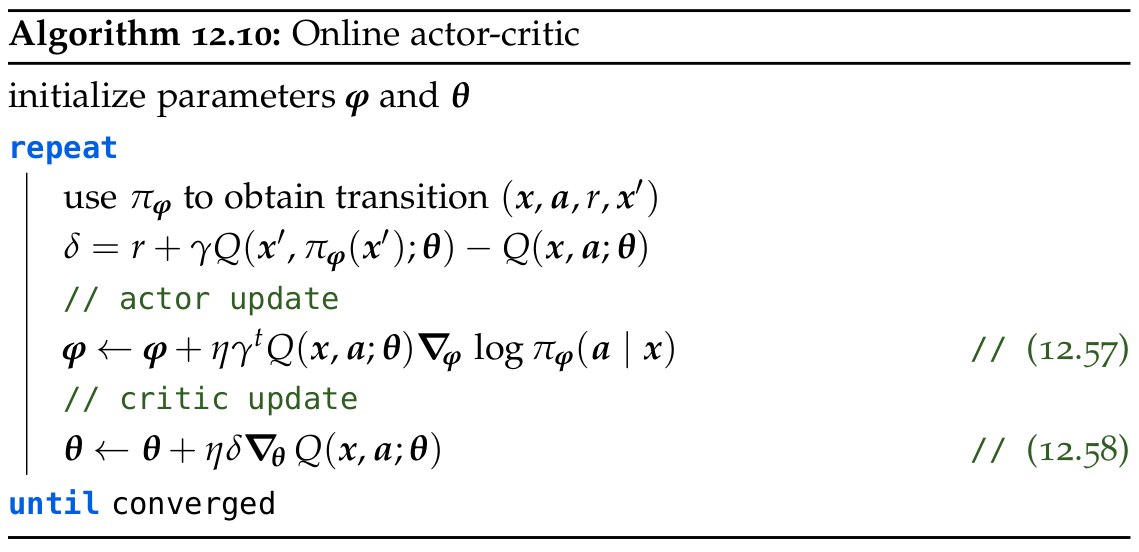
\includegraphics[width=\linewidth]{assets/actor_critic.png}

\begin{definition}[A2C]
    \(Q(x, a; \TH) \to A(x, a; \TH)\) for \(\varphi\)
\end{definition}

\begin{definition}[TRPO]
    Opt. surrogate obj. withing trust region
\end{definition}

\begin{definition}[PPO]
    Effective heuristic variant of TRPO
\end{definition}

\begin{definition}[\color{H2}DDPG]
    Combines DQN with reparam PG
\end{definition}

\begin{definition}[\color{H2}TD3]
    Extension of DDPG to avoid max. bias
\end{definition}

\begin{definition}[\color{H2}SAC]
    Variant of DDPG for \(\Ent\)-regularized MDP
\end{definition}

\begin{definition}[Repa. Policy]
    \(a \sim \pi(x; \TH_\pi) \to a \sim \phi(x; \TH_\pi, \eps)\), deterministic policy + indepenent noise.
\end{definition}
